\chapter{Introduction}

Understanding the human brain is one of the most significant challenges of the 21st century. The brain is responsible

\section{Modern brain imaging}

\begin{figure}[htb]
\begin{center}
   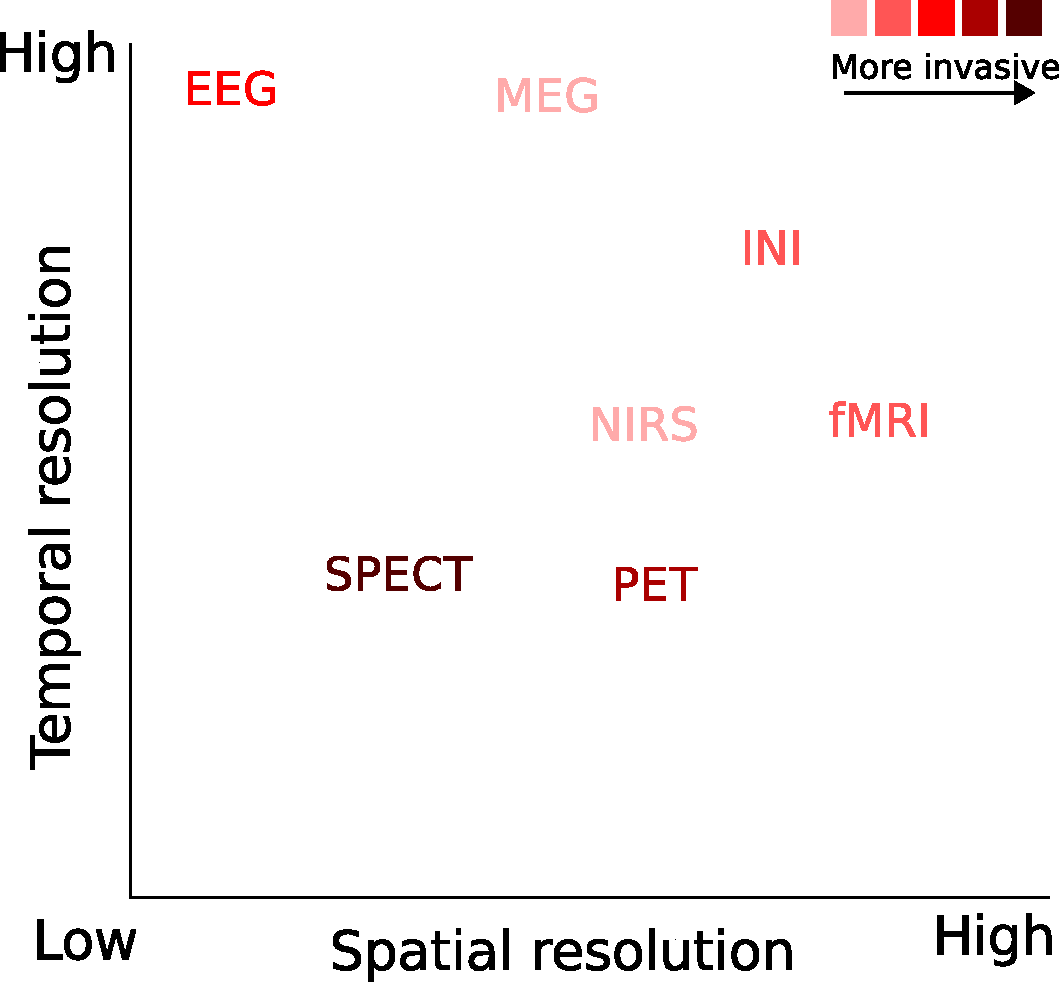
\includegraphics[width=0.4\linewidth]{figures/neuroimaging_methods.pdf}
\end{center}
   \caption[Various neuroimaging methods differ in terms of the information they measure.]{Various neuroimaging methods differ in terms of the information they measure. MEG=magnetoencephalography, EEG=electroencephalography, NIRS=near-infrared spectroscopy, PET=positron emission tomography, SPECT=single photon emission tomography, and INI=Inverse imaging, a method to speed up acquisition of fMRI images.}
   \label{fig:neuroimaging_methods}
\end{figure}

\section{The reproducibility crisis}

Even though thousands of papers are published every year about different aspects of the brain, our understanding of this complex organ has not scaled in proportion. A large part of the reason has been attributed to what is known as the reproducibility crisis~\citep{ioannidis2005most, simmons2011false, button2013power}. %Replication is closely related to the concept of reproducibility which refers to the idea that an experiment produces the same result when performed again under the same conditions. Replication is a stronger condition as it requires similar results or identical conclusion even if there are some minor variations in the experimental procedures. 
Progress in science rests on reproducible experiments. In many fields, however, a large fraction of experiments cannot be reproduced. In psychology, for instance, it was estimated that over half of the papers were not reproducible~\citep{open2015estimating}, and even those which could be reproduced tended to have a weaker effect size compared to the original study. The reasons for unreproducible results can be many, some being: 1) confirmation bias, the tendency to selectively report only experiments that conform to the researcher's pre-existing beliefs, 2) ``p-hacking''~\citep{simmons2011false}, or the tendency to try multiple hypothesis to get a positive result, 3) publication bias or the absence of incentives to publish negative results, and 4) pressure to publish. There are now an accepted set of recommendations to counter many of these issues: 1) pre-registering research plans to avoid confirmation bias and even report negative results, 2) correct for multiple comparisons, the most conservative method being the Bonferroni correction [ref]. 

However, brain imaging has its own set of unique issues which can be linked to reproducibility crisis: 

% vul2009puzzlingly
% yendiki2014spurious

\begin{itemize}[noitemsep,partopsep=0pt]
\item \textbf{Multiple comparison:} Same as in the case of psychology but more widespread due to the presence of large number of voxels or time points [ref]. For instance, in the famous dead salmon study~\citep{bennett2009neural}, an effect was found even if none was expected.
\item \textbf{Differences in software versions:} For instance in the case of Freesurfer software [ref], it can lead to almost a 1 mm [check] difference in cortical thickness~\citep{gronenschild2012effects}.
\item \textbf{Complex pipelines:} Neuroimaging pipelines involve a number of choices at each processing stage, and there isn't currently a consensus on how to choose the right pipeline. Often, these methodological choices are not even documented. It is estimated that almost every new study has its own unique pipeline~\citep{Carp2012289}.
\item \textbf{Power failure:} The statistical power of a study refers to the likelihood of discovering an effect of interest, given the sample size. Small sample sizes translate into underpowered studies which means that the chance of a false discovery is high. In order to discover the effect of interest, the study must be appropriately powered. This is closely related to the problem of multiple comparisons as it is more prevelant in underpowered studies.
\item \textbf{Methodological concerns:} There are several methodological concerns, but perhaps one that has received some attention is the issue of head movements~\citep{yendiki2014spurious} which can lead to spurious correlations.
\end{itemize}

The issue of complex pipelines will be revisited in Chapter []. For now, let us turn our attention to data sharing which can help us alleviate the issue of power failure.

\section{Data sharing}
The history of data sharing can be traced back to Newton and his theory of gravitation~\citep{pointofview2013}. Before Newton had developed his theory, another English astronomer, John Flamsteed had been appointed by the king to observe the stars and produce accurate charts for navigation in the seas. Over a period of 40 years, Flamsteed created a detailed catalogue that tripled the number of entries in the previously used sky atlas. When the great comet of 1680 appeared in the sky twice in close succession, Flamsteed used his data to postulate that it was not two comets but in fact the same comet which first went towards the sun and then turned away from it. Newton initially opposed this theory, but later changed his mind as he gained access to Flamsteed's unpublished catalogue. The comet had indeed turned out to be an important benchmark for Newton's theory of gravitation.

It is hard to imagine in this day and age that a theory as fundamental as the laws of gravitation could have been data driven. Today, data sharing is fundamental to reproducible science, but it also forms the cornerstone for learning better models and benchmarking new algorithms. If one follows the breakthroughs in the field of machine learning, for instance, it is predicated on the availability of data. It is an almost undisputed fact that the recent resurgence of deep learning owes in part at least, to the release of Imagenet~\citep{deng2009imagenet}. The same is true for Q learning in Atari games~\citep{watkins1992q, bellemare2013arcade}, natural language processing for language translation [ref], speech recognition [ref], and even the mixture of experts model~\citep{jacobs1991adaptive} for IBM Watson~\citep{ferrucci2010building}. If such datasets were available in neuroscience, we would be able to tease apart even subtle effects that were not possible before with smaller sample sizes.

Of course, neuroscientists are beginning to realize the importance of sharing data. In recent times, neural data has started being shared through international consortiums~\citep{van2013wu, ollier2005uk} and data repositories~\citep{poldrack2013toward, gorgolewski2015neurovault}. While in the case of Newton, he gained access to the catalogue without permission, today it is possible to publish dataset papers in targeted journals so as to assign the credit where it is due.
Data sharing is beneficial not just from the perspective of replication but also from an economic perspective. Rather than collect new data for every new hypothesis, researchers can now reuse existing data for answering their hypotheses.

\subsection{Brain Imaging Data Structure}

\begin{figure}[htb]
\begin{center}
   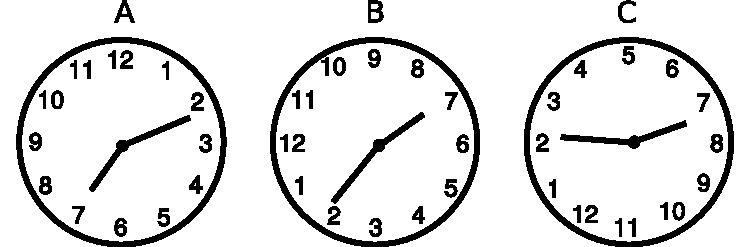
\includegraphics[width=0.8\linewidth]{figures/clock.pdf}
\end{center}
   \caption[Standards in clocks]{Standards in clock design. The time is 07:11 (A) Modern standard, read clockwise and 12 o' clock is at North (B) Anticlockwise and 9 o' clock at North (C) Read clockwise but 5 o' clock is at North. Adapted from \cite{norman2013design}.}
   \label{fig:clock_standards}
\end{figure}

While data sharing in neuroscience is on the rise, the amount of data reuse is still limited. For instance, since the release of the Human Connectome Project (HCP)~\citep{larson2013adding} MEG data in 2013, there have been only one or two documented cases~\citep{jas2017autoreject} of reusing the data. Even in these cases, the effort has mostly been to reproduce rather than test new hypotheses. This clearly represents a gap between the ideal of data sharing and the results in practice. Clearly, sharing data is not a panacea as the tools, skills and resources to process such large datasets is currently missing in typical laboratories. 

Perhaps the most important roadblock is standardization of metadata. Data sharing is clearly not productive if the data is not easily  \emph{reusable} in the same way that uncommented and spaghetti code cannot be reused even if it is shared publicly. Neuroimaging experiments are often complicated involving different paradigms (auditory, visual, somatosensory \emph{etc.}), different acquisition parameters (sampling frequency, number of sensors and their location, measurement device \emph{etc.}), and population parameters: subject's gender, age \emph{etc.} Obviously, this metadata is necessary information to reanalyze the data.   

Unfortunately, there has been historically, a lack of consensus amongst different labs and industrial manufacturer's as to what constitutes useful metadata. This points to the need for establishing standards. While on a superficial glance, this may appear to be unnecessary bureaucratic red tape, the need for standards can be appreciated by considering the simple wall clocks in Figure~\ref{fig:clock_standards}.

The wall clock is recognized as an everyday object that is perhaps far simpler than most complex neuroimaging experiments. Even then, there are two degrees of freedom even to this simple device: the direction of motion of the hands, and the anchor point for the 12 o' clock. While all three clocks in the figure are still readable, it is far more convenient to establish a standard. The upfront cost in conforming to the standard is more than made up by the efficiencies achieved as a result of it.

Apart from the metadata that is stored with the data, the data itself is stored amongst one of 10--20 different file formats and at different stages of processing. While there have been some efforts previously to standardize data structures [ref ESS and neuro without borders], it has not gained wide acceptability. Designing a new standard is tricky as it requires gaining a community consensus. At the same time it must strike the right balance between rigidity for efficiency and flexibility for adapting to future technologies. 

The BIDS format is indeed designed with these considerations in mind. The standard involves a hierarchy of folders to describe the imaging technology used, the name of the subject, and the date of the experiment. At each level of hierarchy, files are accompanied by sidecar \code{json} files describing the metadata. These files follow an inheritance principle, that is, a field described in a \code{json} file in a higher level of the hierarchy will be automatically propagated downstream. The main BIDS specification is accompanied by extension specifications which describe specific aspects of describe certain file types. The BIDS consortium is also providing a growing ecosystem of tools to convert datasets into BIDS compatible format as well as to validate data to conform to the standard. 

The development of these standards is going to enable building large databases of neural recordings. In the future, we can envision being able to open a website and query or search through such data by different experimental paradigms or other metadata.

\section{Automation}
Back in 2014, Nature published a bold article~\citep{hayden2014automated} which described a vision for the future: ``solving the problem of bringing McDonald's-like efficiency to scientists''. This would in turn lead to cheaper, more efficient and reliable research. While it goes on to describe many biology labs which are automating experiments, the benefits of automation in the neuroimaging community are yet to be widely recognized. But what are the opportunities for automation in the context of neuroimaging? Let us list down some of them:
\begin{itemize}[noitemsep,nolistsep,nosep]
\item \textbf{Parameter tuning:} Most algorithms, although automated, require hyperparameters to be tuned. This could be the number of trials to perform in an experiment, the number of components to select in a \ac{PCA} decomposition, or the regularization parameter in inverse solvers.
\item \textbf{Annotation and labeling:} The challenge of neuroimaging data is that it is often unlabeled. As reliable annotations can be performed only by experts, crowdsourcing is often not a possibility. The alternative is to automatically label different types of signals.
\item \textbf{Reporting and quality control:} Automated Statistician . \ac{MNE} web report
\end{itemize}
Ultimately, this will lead to higher quality of 

Efficiency, it turns out, is not simply a matter of scale. Even for moderately sized experiments,

% automated statistician
%
% This subjectivity can lead to studies which are not reproducible unless every single detail was carefully documented. Even then, it does not rule out a potential confirmation bias: the tendency to favor processing steps which leads one to confirm the hypothesis being tested rather than reject it.

data revolution


data sharing, data standards, open source

\subsection{Janitor work}

One of the biggest roadblocks to large scale analysis is what is known as `janitor work': the effort required to standardize a dataset before it is actually usable. In the context of neuroimaging, this can involve organizing files at different stages of processing, manually inspecting the data, annotating segments which contain artifacts, and even removing outlier subjects from the analysis. Merely based on anecdotal reports, we can conclude that this can take up to a week of time even for a moderately sized study of 10--20 subjects.
%If at some point, the researcher realized that a certain parameter early in the pipeline needed to be changed, this would entail redoing all the subsequent steps in the pipeline, including the manual processing. 
In addition to the cost of human labor, one cannot ignore the subjectivity that these steps produces which can be problematic for reproducibility. As the number of datasets shared increases and neuroscientists are forced to confront statistically rigorous approaches to data analysis, the time is ripe to automate as many steps of the pipeline as possible.

\section{Representation learning}
In the last 100 years since the invention of EEG, scientists have discovered several different brain oscillation patterns such as alpha waves, K-complexes, and mu rhythms. The oscillations and interactions between them have served as biomarkers for different brain functions and pathologies. Alpha waves have been implicated in attention, K-complexes in sleep, and mu rhythm in motor activity. However, as these waveforms are buried in the noise, extracting them would require heavy signal processing techniques, particularly those based on Fourier transforms, to emphasize the signal of interest. Obviously, this is not ideal as the sinusoidal bases offered by Fourier transform is not the most compact. A square wave for instance would need to be approximated by a infinite series of sinusoids. Wavelets have therefore been suggested to model the transients. Yet, sinusoidals and wavelets are at best approximations. To best preserve the shape of the waveform, it is necessary to learn the waveform directly from the data. This is the aspiration of representation learning.

In our work, we focus on dictionary learning, a representation learning technique that allows us to learn prototypical `atoms' and their corresponding `activation' maps. As data sharing increases, such a technology is likely to be indispensable as it will allow mining prototypical waveforms on large datasets.

\section{Contributions}
In this thesis, I attempt to synthesize the lessons learned from analysing public neuroimaging data with open source software. To this effect, I participated in an effort to create an MEG standard for the Brain Imaging Data Structure (BIDS)~\citep{galan2017meg}. I wrote the validator which helped create the MEG-BIDS compatible example datasets. As a long time contributor to MNE~\citep{gramfort2013meg}, I led an effort to reanalyze a simple dataset for a reproducible group study. At the same time, we realized that reproducibility cannot be attained unless all steps of analysis pipeline are automated. This led us to develop a fully automated algorithm for artifact rejection and repair~\citep{jas2016automated, jas2017autoreject}. Finally, we develop algorithms to learn new undiscovered motifs automatically from neural time series data. 

\subsection*{Journal publications}
\bibentry{jas2017autoreject} \\ \\
\bibentry{jas2017mne} \\ \\
\bibentry{galan2017meg}

\subsection*{Conference publications}
\bibentry{jas2016automated} \\ \\
\bibentry{jas2017learning}